% $Id: theory.tex 142 2012-12-22 10:41:32Z danbos $
\chapter{Theory}
\label{ch:theory}
In this chapter technologies and topics of relevance for this thesis project work are outlined and explained. It offers a gradual introduction into the technologies and topics applied.

\section{Fuzzy Commitment Scheme}
Traditional cryptographic systems rely on keys, secret sets of bits used for secure management of data. 
For example, a symmetric-key cipher involves a secret key \textit{x} and two operations defined as encryption and decryption.
The encryption function takes as input a message \textit{m} and the key \textit{x} and returns as output a cyphertext \textit{c}.
The decryption function reverses the encryption, taking as input the cyphertext \textit{c} as well as the key and yielding the original message \textit{m}.

Ordinary ciphers rely on exact correctness of the key \textit{x}, making possible the decryption of a cybertext \textit{c} only with a precise key.
Fuzzy commitment, however, is a cryptographic primitive which as has been designed by Juels and Wattenberg \cite{Juels2004AScheme} in order to handle noise over the key \textit{x}.
A commitment scheme is defined as a function $G : C \times X \xrightarrow{} Y$ able to commit a random secret value $\kappa \in C $ choosing a witness $x \in X$ and computing a \textit{blob} value  $y = G(\kappa,x)$.
A decommitment function $G^{-1}: Y \times X \xrightarrow{} C$ takes a blob and a witness as input and yields the original value $\kappa$.
A well defined commitment scheme shall have two basic properties:
\begin{itemize}
    \item binding: it is not possible to decommit $y$ under a pair $(\kappa', x')$ such that $\kappa' \neq \kappa$ ;
    \item hiding: given $y$ alone, it is infeasible to compute $\kappa$.
\end{itemize}
The fuzzy commitment encryption scheme allows the recovery of $\kappa$ from a given commitment $y=G(\kappa, x)$ from any witness $x'$ close to $x$ in some appropriate metric, such as Hamming distance, but not necessarily identical to $x$.
Since $h(c)$ is a secure one-way function, $y$ leaks only a small amount of information about a committed value, therefore it may be revealed publicly and used to recover $\kappa$ using any close witness $x'$.

The $n$-bit witness can be expressed  in terms of the committed value with an $n$-bit offset $\delta$ such that $x = \kappa \oplus \delta$. The idea behind the commitment function $G$ is to hide $\kappa$ using an hash function $h$ (such as SHA256) while leaving $\delta$ in clear. 
The commitment function can be then defined as:
\begin{center}
    $G(\kappa,x) = (h(\kappa), x \oplus \kappa) = (h(\kappa), \delta)$
\end{center}
It is then possible to leverage the error correcting properties of error correcting codes such as \ac{RS} to correctly recover the secret $\kappa$.
An error-correcting code comprises a message space $C \subseteq \{0,1\}^a$ , a corresponding codeword space $C \subseteq \{0,1\}^b$ , for $b \geq a$, and a bijection $\varphi : M \longleftrightarrow C$. 
Here $\{ 0, 1 \}^k$ denotes a $k$-bit message/codeword generating a space with a total of $2^k$ distinct elements.
Another important element of error-correcting codes is a decoding function $f:C' \xrightarrow{} C \cup \bot$, where $C \subseteq C' \subseteq \{0,1\}^b $.
The role of the decoding function is to map an element in $C'$ to its nearest (i.e., nearest in terms of Hamming distance) element in $C$, resulting in the elimination of the noise added to a codeword or the failure to find a valid one, denoted with the symbol $\bot$.


To decommit $F(\kappa,\delta)$ using a witness $x'$ , the receiver computes $\kappa ' = f(x' \oplus \delta)$ , where $f$ is an efficient decoding function from the error correcting code.
If the received $h(\kappa)$ corresponds to $h(\kappa ')$ then the blob has been successfully decommitted, with $\kappa '$ representing the extracted commitment, otherwise, $x'$ represents an incorrect witness. 

One application of fuzzy commitment, as suggested by the authors in \cite{Juels2004AScheme}, is to secure biometric systems.
An enrolled fingerprint image (known as a template), for example, might be viewed as a key $x$. The user tries to authenticate using another, slightly different image of the same finger,which we may denote by $x'$. Authentication is successful if and only if $x'$ is "close" to $x$.

%%%Fuzzy extractors are used to convert biometric data into random strings which can be applied in cryptographic techniques for biometric security. 
%One of the first fuzzy extractors systems is \textit{Fuzzy commitment} \cite{Juels2004AScheme}, designed by Juels and Wattenberg, where, using biometric data "close" to each others, is possible to decommit a cryptographic key.
%The idea is to bind a string of random bits with a biometric template in binary format called difference vector.
%Ideally, it is infeasible to recover the difference vector either the biometric template or the random bit string without any knowledge of the user's biometric data.

\section{Elliptic Curves Cryptography}
\label{theory:ECC}
Elliptic curve cryptography is a public key cryptosystem developed by Neil Kobiltz and Victor Miller in 19th century \cite{Miller2000TheCryptography}.
An elliptic curve (\acs{EC}) over the field $\mathbb{F}$ is the set of all solutions (x,y) in $\mathbb{F}$ that satisfy the mathematical equation:
\begin{equation}
y^2 + a_1xy + a_3 y = x^3 + a_2 x^2 + a_4 x + a_6
\end{equation}
where $a_1,a_2,a_3,a_4,a_5,a_6 \in \mathbb{F}$ together with a point at \textit{infinity} denoted by $\infty$.
Cryptographic systems usually use elliptic curves over prime fields $\mathbb{F}_p$ ( for some large prime number $p$) or binary fields ($\mathbb{F}^m_2$ for some integer $m$ ), since field arithmetic in these particular fields can be implemented very efficiently. 
For the purpose of this thesis, we have focused on prime field curves recommended by the National Institute of Standards and Technology (NIST) using implementation following these standard practices. 
In curves over a prime field, the \textit{Weierstrass} equation above can be expressed, using a variable change, as a much simpler equation of the form

\begin{equation}
y^2 = x^3 + ax + b
\label{ec_formula}
\end{equation}

The set of points $x,y \in \mathbb{F}$ that satisfy equation \ref{ec_formula}, plus the point $\infty$ and an "addition" form a group \cite{Washington2008EllipticApplications}.
To perform the operation of addition of two points $\mathbb{P}(x_1,y_1) \neq \mathbb{Q}(x_2,y_2) $ and  $ \mathbb{P},\mathbb{Q}\neq \infty$ on the curve $E(a, b)$ to obtain a third point $R(x_3, y_3)$ on the curve, we need draw a straight line that passes through the two points. 
The line will intersect the curve in another point $-\mathbb{R}$. 
Reflecting across the x-axis that point, we find the third point, $\mathbb{R}$, as shown in Figure \ref{fig_ec}. 

\begin{figure}[!h]
\centering
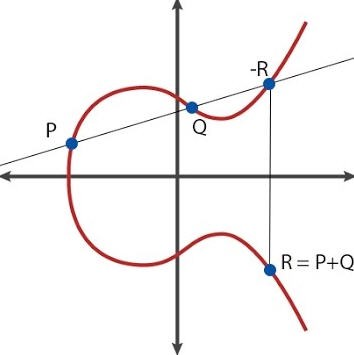
\includegraphics[width=3in]{images/ecc.png}
\caption{Group law on an elliptic curve.}
\label{fig_ec}
\end{figure}

In the case where $\mathbb{P} = \mathbb{Q}$, we will draw a line tangent to that point and then looking for the point which intersects with the curve. Its reflection along the x-axis is the sum $\mathbb{P} + \mathbb{P}$.
If $\mathbb{P} = \mathbb{Q}$ with $y=0$ or $y_1 \neq y_2$, the sum will be $\mathbb{P} + \mathbb{Q} = \infty$.
A related group operation is the scalar point multiplication, where by a given point is added to itself a given number of times.

The security of elliptic curve cryptography rests on the assumption that the \ac{ECDLP} is hard, which represent the fundamental building block for \acs{ECC}.
The ECDLP is the following computational problem:
given points $\mathbb{P}, \mathbb{Q} \in \mathbb{E}$ to find an integer $a$, if it exists, such that $\mathbb{Q} = a \mathbb{P}$.

Elliptic Curve Cryptography (ECC) is a preferred choice among various PKC options due to its fast computation, small key size, and compact signatures\cite{Research2000}. 
Experiments proved that Elliptic Curve Cryptography (ECC) is more suitable for resource constraint devices compared with RSA \cite{Gura2004}\cite{2005EnergyNetworks}.
For example, to provide equivalent security to 1024-bit RSA, an ECC scheme only needs 160 bits on various parameters, such as 160-bit finite field field operations and 160-bit key size\cite{Research2000}. 
EC parameters are denoted by \textit{a, b, q, p and $\mathbb{P}$} and they are embedded in all the entities that participate in the communication scenario. 
The parameter q is the prime which indicates the finite field $\mathbb{F}_q$. 
The variables $a$ and $b$ are the coefficients of the elliptic curve. 
$\mathbb{P}$ is the base point generator with order $p$ which is a  prime number.

\section{One Way Accumulators}
%We build a secure group membership operation by using one-way accumulators \cite{10.1007/3-540-48285-7_24} using point multiplication on elliptic curve as a one-way asymmetric accumulator. 
%\begin{center}
%$f(s,\mathbb{P}) = s \times \mathbb{P} = \mathbb{Q}$
%\end{center}
%where $\mathbb{P}$ and $\mathbb{Q}$ are points on the curve and $s$ is a large scalar value.
The concept of one-way accumulator, proposed by Benaloh and Mare \cite{10.1007/3-540-48285-7_24}, was designed mainly for timestamping purposes and memberhip testing. 
A cryptographic one-way accumulator is a way to combine a set of values into one accumulator value, in such a way that, all the entities which participated in the generation of this accumulator value with their values are able to produce a witness.
Over time, other applications such as distributed signatures and accountable certificate management \cite{Buldas2004AccountableAttestations} have been proposed.
Formally, a one-way accumulator is essentially a one-way hash function $f : \mathbb{X} \times \mathbb{Y} \xrightarrow{} \mathbb{X}$ with the quasi-commutative property:
\begin{equation}
    \forall x \in \mathbb{X}, \forall y_1,y_2 \in \mathbb{Y} : f(f(x,y_1), y_2) = f(f(x,y_2), y_1)
\end{equation}
This hash function can be used to compute an accumulator value $z$ starting from an initial value $x \in \mathbb{X}$ and for all the values in $y_1,...,y_n \in \mathbb{Y}$ by applying $f$ repeatedly to each value $y_i$. 
The hash function can ensure that the accumulator value does not depend on the order in which the items participating in its generation appears.
The one-way accumulator can be also used  to generate a witness $z_j$ for a value $y_j$ in $\mathbb{Y}$ by hashing all elements $y_i \in \mathbb{Y}$ such as $i \neq j$. 
Using the quasi-commutative property of $f$ it is possible to recover $z = f(z_j,y_j), \forall y_j \in \mathbb{Y}$.

In this thesis has been used point multiplication on elliptic curve as a one-way asymmetric accumulator to generate a witness and to establish a group key.
Given a curve $E$, the function $f$ is defined as:
\begin{equation}
    f(\mathbb{P},s) = \mathbb{P} \times s = \mathbb{Q}
\end{equation}
where, given a base point $\mathbb{P} \in E$ and a scalar integer $s$, $f$ computes the scalar multiplication to find a new point $\mathbb{Q} \in E$. Due to the ECDLP, this operation results one-way because, given the two points $\mathbb{P}$ and $\mathbb{Q}$, it is hard to compute the scalar value $s$. 
The function $f$ results quasi-commutative since we have:
\begin{equation}
    f(f(\mathbb{P},s_1),s_2) = f(f(\mathbb{P},s_2),s_1) = \mathbb{P} \times (s_1 s_2) 
\end{equation}



\section{Related work}
\iffalse
In recent, years biometric information is utilised to an in-creasing degree to replace or enhance classical cryptographic schemes \cite{Skoric2010SecurityData}.  Popular examples are photos or finger prints in ID-documents, Iris-scans or in the future probably short tandem repeats in a human’s DNA [29].  Generally, features are extracted from the biometric data and a characteristic set of features is required to match in o
\fi

The proposed protocol is based on a previous work presented in \cite{Gebremichael2018} and \cite{Ferrari2018}.
There are well studied group key establishment protocols in use today. 
An extension of the Diffie-Hellman protocol to a group of nodes with the generation of a one-time session key is described in \cite{Steiner1996}and \cite{Bresson2007}. However, the intensive computational power required for the execution of these protocols makes them not ideal for power and resources constrained devices.
Moreover, \cite{Bohli2007} demonstrated that \cite{Bresson2007} does not meet some security requirements.

A conference-key distribution system is proposed in \cite{Ingemarsson1982} but the the system resulted insecure because the information exchanged by the users makes it possible for a passive eavesdropper to compute the key. 
Moreover, the approach used for \cite{Ingemarsson1982}  requires a high number of messages exchanged and an high number of expensive computational operations.

Some of the earliest proposed protocols such as $\mu$TESLA \cite{Perrig2002} belongs to the symmetric key based protocols category and they are based on hash function in order to reduce the energy consumption. 
Other symmetric key schemes based on key ring like \cite{Bohli2007} are not scalable, and therefore, these are unsuitable for dynamic environments such in the analyzed scenario.

In \cite{Porambage2015} the authors propose two lightweight group-key establishment protocols using an approach similar to ours.
The first protocol allows only the legitimate members of the multicast group as eligible to continue the rest of the process of key derivation. 
This one is more appropriate for distributed IoT applications, which require nodes to contribute hightly to the key computation and need greater randomness. 
The second one allows to establish a shared secret key among the multicast group. This one is more suitable for centralized IoT applications, where a central entity performs the  majority of the cryptographic functions. 

For the purpose of authentication, most of the proposed solutions involve human interaction such as the Wi-Fi protected setup \cite{EldefrawyDynamicTimestamping} or the the necessity to use pre shared keys such as \cite{Gebremichael2019LightweightPad}. 
In recent, years biometric information is utilised to an in-creasing degree to replace or enhance classical cryptographic schemes \cite{Skoric2010SecurityData}.
Researchers started to explore context-based pairing protocol in order to capture commonly observed context features for pairing, leveraging on-board sensors and removing the "human-in-the-loop" factor.
A solution which uses ambient light or sound is proposed in \cite{Miettinen2014Context-BasedDescriptors}. 
In \cite{Schurmann2013SecureAudio} is proposed a solution which leverages audio for the secure pairing, but it results sensible to synchronization.
A solution based on heterogeneous context features is proposed in  \cite{Han2018DoTypes} and it relies on events observed by each sensor.





